\documentclass[xcolor=x11names,compress,bigger]{beamer}

%% General document %%%%%%%%%%%%%%%%%%%%%%%%%%%%%%%%%%
\usepackage[utf8]{inputenc}
\usepackage[T1]{fontenc}
\usepackage{hyperref}
\usepackage[english,nynorsk]{babel}
\usepackage{apacite} % after babel
\usepackage{natbib}
\usepackage{pslatex}

\usepackage{enumerate}
\usepackage{subfigure}
\usepackage{linguex}

\def\newblock{\hskip .11em plus .33em minus .07em} % for using bibtex with beamer 

\usepackage{graphicx}
\usepackage{tikz}
\usepackage{tikz-qtree}
\usepackage{avm}
\avmfont{\sc}
\avmoptions{sorted,active}
\avmvalfont{\rm}
\avmsortfont{\scriptsize\it}
\usetikzlibrary{calc}

%% My own commands %%%%%%%%%%%%%%%%%%%%%%%%%%%%%%%%%%%
\newcommand{\mytilde}{\raise.17ex\hbox{$\scriptstyle\sim$}}
\newcommand{\xbar}{$\rm\overline{X}$}
\newcommand{\ind}[1]{{\avmoptions{center}\begin{avm}\@{#1}\end{avm}}}
\newcommand{\F}[2]{\textsc{#1}\ensuremath{_{#2}}}
\newcommand{\q}[2]{\begin{quotation}\raggedleft{}#1\\\vspace{0.2cm}(#2)\vspace{1.2cm}\end{quotation}}
\newcommand{\OBLben}{\F{obl}{ben}}
\newcommand{\OBJben}{\F{obj}{ben}}
\newcommand{\OBJ}{\F{obj}{}}
\newcommand{\OBJs}{\F{obj~}{}}
\newcommand{\ADJ}{\F{adj}{}}
\newcommand{\ADJs}{\F{adj~}{}}
\newcommand{\ADJUNCT}{\F{adjunct}{}}
\newcommand{\XCOMP}{\F{xcomp}{}}
\newcommand{\XCOMPs}{\F{xcomp~}{}}
\newcommand{\SUBJ}{\F{subj}{}}
\newcommand{\SUBJs}{\F{subj~}{}}
\newcommand{\SPEC}{\F{spec}{}}
\newcommand{\POSS}{\F{poss}{}}
\newcommand{\GEND}{\F{gend}{}}
\newcommand{\NUM}{\F{num}{}}
\newcommand{\PRED}{\F{pred}{}}
\newcommand{\TOPIC}{\F{topic}{}}
\newcommand{\falign}{\ensuremath{\operatorname{\emph{falign}}}}
\newcommand{\fpairs}{\ensuremath{\operatorname{\emph{fpairs}}}}
\newcommand{\Bleu}{\textsc{Bleu}}
\newcommand{\proj}[2]{\begin{tabular}{c}\footnotesize{#1}\\\normalsize{#2}\end{tabular}}
\newcommand{\ua}{\ensuremath{\uparrow}}
\newcommand{\da}{\ensuremath{\downarrow}}
\newcommand{\p}[1]{`\textbf{#1}'}
\renewcommand{\BOthers}{mfl.\hbox{}}
\renewcommand{\BOthersPeriod}{mfl.\hbox{}}


%%%%%%%%%%%%%%%%%%%%%%%%%%%%%%%%%%%%%%%%%%%%%%%%%%%%%%


%% Beamer Layout %%%%%%%%%%%%%%%%%%%%%%%%%%%%%%%%%%
\useoutertheme[subsection=false,shadow]{miniframes}
\useinnertheme{default}
\usefonttheme{serif}
\usepackage{palatino}

\setbeamerfont{title like}{shape=\scshape}
\setbeamerfont{frametitle}{shape=\scshape}

\setbeamercolor*{lower separation line head}{bg=DeepSkyBlue4} 
\setbeamercolor*{normal text}{fg=black,bg=white} 
\setbeamercolor*{alerted text}{fg=red} 
\setbeamercolor*{example text}{fg=black} 
\setbeamercolor*{structure}{fg=black} 
 
\setbeamercolor*{palette tertiary}{fg=black,bg=black!10} 
\setbeamercolor*{palette quaternary}{fg=black,bg=black!10} 

\renewcommand{\(}{\begin{columns}}
\renewcommand{\)}{\end{columns}}
\newcommand{\<}[1]{\begin{column}{#1}}
\renewcommand{\>}{\end{column}}
%%%%%%%%%%%%%%%%%%%%%%%%%%%%%%%%%%%%%%%%%%%%%%%%%%



\begin{document}

%%%%%%%%%%%%%%%%%%%%%%%%%%%%%%%%%%%%%%%%%%%%%%%%%%%%%%
%%%%%%%%%%%%%%%%%%%%%%%%%%%%%%%%%%%%%%%%%%%%%%%%%%%%%%
\begin{frame}[plain]
  \title[Syntaktisk fraselenking]{
    \scalebox{1.0}{\centering\scriptsize{}\avmoptions{}
      \begin{tikzpicture}[scale=0.5]
        \node(src){
          \begin{avm}
            \[ adjunct & \[ `{\bf{}syntaktisk}' \]  \\
               pred  & `{\bf{}fraselenking}' \]
          \end{avm}
        };
        \node[below of=src, node distance=2cm](trg){
          \begin{avm}
            \[pred   &  `{\bf{}link}'\\
            adjunct & \[ `{\bf{}of<\@{1}>}' \\
                          obj & \@{1} \[ adjunct & \[ `{\bf{}syntactic}' \] \\
                                         pred `{\bf{}phrase}' 
            \] \] \]
          \end{avm}
        };
        \draw[-] ($(src.south)+(0.0,+0.2)$) .. controls +(-0,-1.5) and +( 0,1.5) .. ($(trg.west) +( 4.0,2.0)$) ;
        \draw[-] ($(src.south)+(0.0,+0.2)$) .. controls +(-0,-1.5) and +( 0,1.5) .. ($(trg.south)+( 2.5,1.0)$) ;
        \draw[-] ($(src.north)+(2.0,-0.4)$) .. controls +(3.1,2.1) and +(-1,1.5) .. ($(trg.east) +(-2.5,0.0)$) ;
      \end{tikzpicture}
    }
  }
    \author{\small
  Kevin Brubeck Unhammer}
    \institute{ Universitetet i Bergen}
  \date{\small
    10. desember 2010}
  \titlepage
\end{frame}

\begin{frame}
  \tableofcontents
\end{frame}

%%%%%%%%%%%%%%%%%%%%%%%%%%%%%%%%%%%%%%%%%%%%%%%%%%%%%%
%%%%%%%%%%%%%%%%%%%%%%%%%%%%%%%%%%%%%%%%%%%%%%%%%%%%%%
\section{\scshape Fraselenking}
\subsection{Kva og kvifor}
\begin{frame}\frametitle{Fraselenking}
    \begin{itemize}
    \item Finne frasar som korresponderer i omsetjingar
      \begin{itemize}
      \item  «frase» = konstituent? dependenseining?
        syntaktisk funksjon? N-gram? chunk?
      \end{itemize}
    \item Data: vanlegvis N-gramtabellar frå statistisk samanstilling,
      reint korpusbasert
    \item Formål: vanlegvis statistisk maskinomsetjing
    \end{itemize}
\end{frame}

\subsection{Standardmetoden: N-grambasert}
\begin{frame}[fragile]
  \begin{tikzpicture}[auto]
       \tikzstyle{frame} = [rectangle, draw=blue, thick, fill=blue!20];
       \matrix [row sep=1cm,column sep=0.5cm,ampersand replacement=\&]
       {
         \node(there){There}; \&
         \node('s){'s}; \&
         \node(an){an}; \&
         \node(elephant){elephant}; \&
         \node(in){in}; \&
         \node(the){the}; \&
         \node(room){room};\\[1cm]
         \node(es){Es}; \&
         \node(gibt){gibt}; \&
         \node(ein){ein}; \&
         \node(elefant){Elefant}; \&
         \node(im){im}; \&
         \node(raum){Raum}; \\
         \& % Es
         \& % gibt
         \& % ein
         \node(X'){~}; \& % Elefant
         \& % im
         \& \\% Raum
         \& % Es
         \& % gibt
         \node(XP){~}; \& % ein
         \& % Elefant
         \& % im
         \& \\% Raum
       };      
       \draw[-] ($(there.south)+(0.0,0.0)$) .. controls +(0,0) and +(0,0) .. ($('s.south) +(0.0,0.0)$) ;
       \draw[-] ($(es.north)+(0.0,0.0)$) .. controls +(0,0) and +(0,0) .. ($(gibt.north) +(0.0,0.0)$) ;
       \draw[-] ($(there.south)+(0.0,0.0)$) .. controls +(0,0) and +(0,0) .. ($(es.north) +(0.0,0.0)$) ;
       \draw[-] ($('s.south)+(0.0,0.0)$) .. controls +(0,0) and +(0,0) .. ($(gibt.north) +(0.0,0.0)$) ;

       \draw[-] ($(an.south)+(0.0,0.0)$) .. controls +(0,0) and +(0,0) .. ($(elephant.south) +(0.0,0.0)$) ;
       \draw[-] ($(ein.north)+(0.0,0.0)$) .. controls +(0,0) and +(0,0) .. ($(elefant.north) +(0.0,0.0)$) ;
       \draw[-] ($(an.south)+(0.0,0.0)$) .. controls +(0,0) and +(0,0) .. ($(ein.north) +(0.0,0.0)$) ;
       \draw[-] ($(elephant.south)+(0.0,0.0)$) .. controls +(0,0) and +(0,0) .. ($(elefant.north) +(0.0,0.0)$) ;

       \draw[-] ($(in.south)+(0.0,0.0)$) .. controls +(0,0) and +(0,0) .. ($(room.south) +(0.0,0.0)$) ;
       \draw[-] ($(im.north)+(0.0,0.0)$) .. controls +(0,0) and +(0,0) .. ($(raum.north) +(0.0,0.0)$) ;
       \draw[-] ($(in.south)+(0.0,0.0)$) .. controls +(0,0) and +(0,0) .. ($(im.north) +(0.0,0.0)$) ;
       \draw[-] ($(room.south)+(0.0,0.0)$) .. controls +(0,0) and +(0,0) .. ($(raum.north) +(0.0,0.0)$) ;
     \end{tikzpicture}
\end{frame}

\begin{frame}[fragile]
  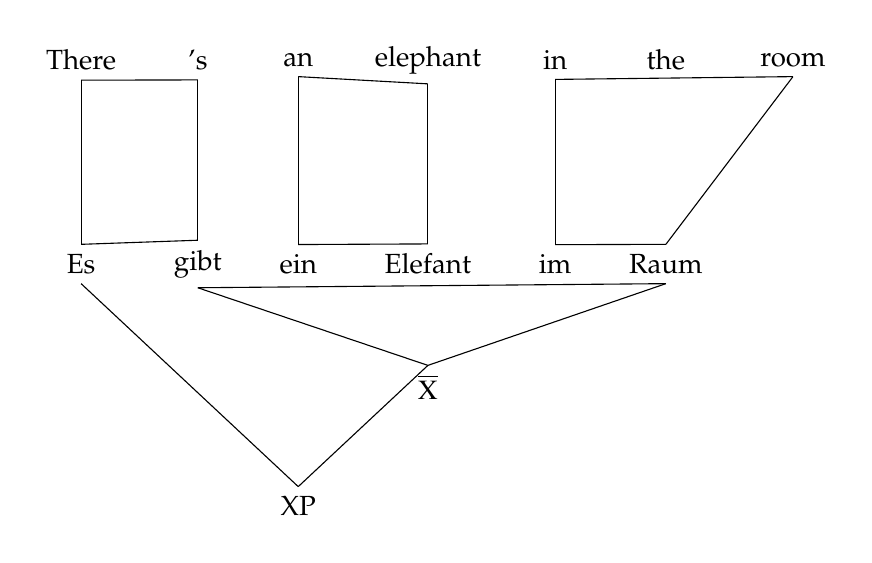
\begin{tikzpicture}[auto]
       \tikzstyle{frame} = [rectangle, draw=blue, thick, fill=blue!20];
       \matrix [row sep=1cm,column sep=0.5cm,ampersand replacement=\&]
       {
         \node(there){There}; \&
         \node('s){'s}; \&
         \node(an){an}; \&
         \node(elephant){elephant}; \&
         \node(in){in}; \&
         \node(the){the}; \&
         \node(room){room};\\[1cm]
         \node(es){Es}; \&
         \node(gibt){gibt}; \&
         \node(ein){ein}; \&
         \node(elefant){Elefant}; \&
         \node(im){im}; \&
         \node(raum){Raum}; \\
         \& % Es
         \& % gibt
         \& % ein
         \node(X'){\xbar}; \& % Elefant
         \& % im
         \& \\% Raum
         \& % Es
         \& % gibt
         \node(XP){XP}; \& % ein
         \& % Elefant
         \& % im
         \& \\% Raum
       };      
       \draw[-] ($(there.south)+(0.0,0.0)$) .. controls +(0,0) and +(0,0) .. ($('s.south) +(0.0,0.0)$) ;
       \draw[-] ($(es.north)+(0.0,0.0)$) .. controls +(0,0) and +(0,0) .. ($(gibt.north) +(0.0,0.0)$) ;
       \draw[-] ($(there.south)+(0.0,0.0)$) .. controls +(0,0) and +(0,0) .. ($(es.north) +(0.0,0.0)$) ;
       \draw[-] ($('s.south)+(0.0,0.0)$) .. controls +(0,0) and +(0,0) .. ($(gibt.north) +(0.0,0.0)$) ;

       \draw[-] ($(an.south)+(0.0,0.0)$) .. controls +(0,0) and +(0,0) .. ($(elephant.south) +(0.0,0.0)$) ;
       \draw[-] ($(ein.north)+(0.0,0.0)$) .. controls +(0,0) and +(0,0) .. ($(elefant.north) +(0.0,0.0)$) ;
       \draw[-] ($(an.south)+(0.0,0.0)$) .. controls +(0,0) and +(0,0) .. ($(ein.north) +(0.0,0.0)$) ;
       \draw[-] ($(elephant.south)+(0.0,0.0)$) .. controls +(0,0) and +(0,0) .. ($(elefant.north) +(0.0,0.0)$) ;

       \draw[-] ($(in.south)+(0.0,0.0)$) .. controls +(0,0) and +(0,0) .. ($(room.south) +(0.0,0.0)$) ;
       \draw[-] ($(im.north)+(0.0,0.0)$) .. controls +(0,0) and +(0,0) .. ($(raum.north) +(0.0,0.0)$) ;
       \draw[-] ($(in.south)+(0.0,0.0)$) .. controls +(0,0) and +(0,0) .. ($(im.north) +(0.0,0.0)$) ;
       \draw[-] ($(room.south)+(0.0,0.0)$) .. controls +(0,0) and +(0,0) .. ($(raum.north) +(0.0,0.0)$) ;

       \draw[-] ($(es.south)+(0.0,0.0)$) .. controls +(0,0) and +(0,0) .. ($(XP.north) +(0.0,0.0)$) ;
       \draw[-] ($(XP.north)+(0.0,0.0)$) .. controls +(0,0) and +(0,0) .. ($(X'.north) +(0.0,0.0)$) ;
       \draw[-] ($(X'.north)+(0.0,0.0)$) .. controls +(0,0) and +(0,0) .. ($(gibt.south) +(0.0,0.0)$) ;
       \draw[-] ($(X'.north)+(0.0,0.0)$) .. controls +(0,0) and +(0,0) .. ($(raum.south) +(0.0,0.0)$) ;
       \draw[-] ($(gibt.south)+(0.0,0.0)$) .. controls +(0,0) and +(0,0) .. ($(raum.south) +(0.0,0.0)$) ;
     \end{tikzpicture}
\end{frame}

\begin{frame}[fragile]
  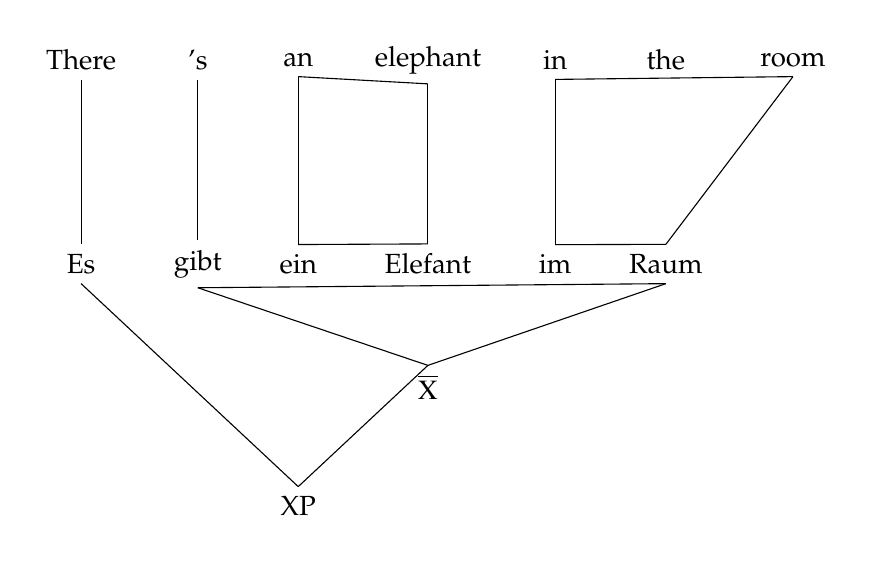
\begin{tikzpicture}[auto]
       \tikzstyle{frame} = [rectangle, draw=blue, thick, fill=blue!20];
       \matrix [row sep=1cm,column sep=0.5cm,ampersand replacement=\&]
       {
         \node(there){There}; \&
         \node('s){'s}; \&
         \node(an){an}; \&
         \node(elephant){elephant}; \&
         \node(in){in}; \&
         \node(the){the}; \&
         \node(room){room};\\[1cm]
         \node(es){Es}; \&
         \node(gibt){gibt}; \&
         \node(ein){ein}; \&
         \node(elefant){Elefant}; \&
         \node(im){im}; \&
         \node(raum){Raum}; \\
         \& % Es
         \& % gibt
         \& % ein
         \node(X'){\xbar}; \& % Elefant
         \& % im
         \& \\% Raum
         \& % Es
         \& % gibt
         \node(XP){XP}; \& % ein
         \& % Elefant
         \& % im
         \& \\% Raum
       };      
       \draw[-] ($(there.south)+(0.0,0.0)$) .. controls +(0,0) and +(0,0) .. ($(es.north) +(0.0,0.0)$) ;
       \draw[-] ($('s.south)+(0.0,0.0)$) .. controls +(0,0) and +(0,0) .. ($(gibt.north) +(0.0,0.0)$) ;

       \draw[-] ($(an.south)+(0.0,0.0)$) .. controls +(0,0) and +(0,0) .. ($(elephant.south) +(0.0,0.0)$) ;
       \draw[-] ($(ein.north)+(0.0,0.0)$) .. controls +(0,0) and +(0,0) .. ($(elefant.north) +(0.0,0.0)$) ;
       \draw[-] ($(an.south)+(0.0,0.0)$) .. controls +(0,0) and +(0,0) .. ($(ein.north) +(0.0,0.0)$) ;
       \draw[-] ($(elephant.south)+(0.0,0.0)$) .. controls +(0,0) and +(0,0) .. ($(elefant.north) +(0.0,0.0)$) ;

       \draw[-] ($(in.south)+(0.0,0.0)$) .. controls +(0,0) and +(0,0) .. ($(room.south) +(0.0,0.0)$) ;
       \draw[-] ($(im.north)+(0.0,0.0)$) .. controls +(0,0) and +(0,0) .. ($(raum.north) +(0.0,0.0)$) ;
       \draw[-] ($(in.south)+(0.0,0.0)$) .. controls +(0,0) and +(0,0) .. ($(im.north) +(0.0,0.0)$) ;
       \draw[-] ($(room.south)+(0.0,0.0)$) .. controls +(0,0) and +(0,0) .. ($(raum.north) +(0.0,0.0)$) ;

       \draw[-] ($(es.south)+(0.0,0.0)$) .. controls +(0,0) and +(0,0) .. ($(XP.north) +(0.0,0.0)$) ;
       \draw[-] ($(XP.north)+(0.0,0.0)$) .. controls +(0,0) and +(0,0) .. ($(X'.north) +(0.0,0.0)$) ;
       \draw[-] ($(X'.north)+(0.0,0.0)$) .. controls +(0,0) and +(0,0) .. ($(gibt.south) +(0.0,0.0)$) ;
       \draw[-] ($(X'.north)+(0.0,0.0)$) .. controls +(0,0) and +(0,0) .. ($(raum.south) +(0.0,0.0)$) ;
       \draw[-] ($(gibt.south)+(0.0,0.0)$) .. controls +(0,0) and +(0,0) .. ($(raum.south) +(0.0,0.0)$) ;
     \end{tikzpicture}
\end{frame}

\begin{frame}\frametitle{\texttt{\normalsize cat n-gramtabell | fraselenking | syntaks}}
    \begin{itemize}
    \item N-grambasert (datadriven/korpusbasert) lenking kan filtrerast med kunnskap
      \begin{itemize}
       \item berre lenkjer som samsvarer med syntaktiske nodar \citep{samuelsson2007apa}
       \item berre lenkjer som samsvarer med ein dependensanalyse \citep{hearne2008ccd}
       \item berre lenkjer som samsvarer med ein f-strukturanalyse \citep{graham2009osr}
      \end{itemize}
    \end{itemize}
  \end{frame}

\begin{frame}\frametitle{\texttt{\normalsize cat syntaks | fraselenking | n-gramtabell}}
  \begin{itemize}
  \item Men me kan au gå andre vegen
    \begin{itemize}
    \item Data: LFG-analysar
    \item Formål: annotert trebank
    \item Kunnskapsdriven lenking, kan ev. filtrerast med N-gramtabell
      (eller omsetjingsordbok)
    \end{itemize}
  \end{itemize}
\end{frame}

%%%%%%%%%%%%%%%%%%%%%%%%%%%%%%%%%%%%%%%%%%%%%%%%%%%%%%
%%%%%%%%%%%%%%%%%%%%%%%%%%%%%%%%%%%%%%%%%%%%%%%%%%%%%%
\section{\scshape Lenkingskrav}
\subsection{F-strukturlenkjer}

\begin{frame}
  \begin{tikzpicture}
     {\avmoptions{}
      \node(src){
         \begin{avm}
           $f$ \[pred  & `{\bf{}sove}<eg>' \\
           tense & pret \\
           ... \]
         \end{avm}
       };
       \node[right of=src, node distance=5cm](trg){
         \begin{avm}
           $g$ \[pred   &  `{\bf{}sleep}<I>'\\
           tense  & pret  \\
           aspect & simple \\
           ... \]
         \end{avm}
       };
       }
%       \draw[dashed,-] (src.west) .. controls +(-1,2) and +(-1,2) .. node[above,sloped]{$l_f$} (trg.west) ;
       %\draw[-] ($(src.north)-(1,0.3)$) .. controls +(0,1.5) and +(0,1.5) .. node[above,sloped]{$l_p$} ($(trg.north)-(1,0.3)$) ;
  
       \begin{scope}[shift={(0,-3cm)}]
      \Tree  [.\node(VPs){VP}; [.\node(Vs){\proj{\ua =\da}{V}}; \node(sov){sov};  ] ]
       \begin{scope}[shift={(5cm,0)}]
         \Tree  [.\node(VPt){VP}; [.\node(Vt){\proj{\ua =\da}{V}}; \node(slept){slept};  ] ]
       \end{scope}
       \end{scope}
       %\draw[-] (VPs)..controls +(north:1.5) and +(north:1.5) .. node[above,sloped]{$l_c$} (VPt) ;
%       \draw[dashed,-] (sov)..controls +(north east:1.5) and +(north west:1.5) .. node[above,sloped]{$l_o$} (slept) ;
    \end{tikzpicture}
\end{frame}

\begin{frame}
  \begin{tikzpicture}
     {\avmoptions{}
      \node(src){
         \begin{avm}
           $f$ \[pred  & `{\bf{}sove}<eg>' \\
           tense & pret \\
           ... \]
         \end{avm}
       };
       \node[right of=src, node distance=5cm](trg){
         \begin{avm}
           $g$ \[pred   &  `{\bf{}sleep}<I>'\\
           tense  & pret  \\
           aspect & simple \\
           ... \]
         \end{avm}
       };
       }
%       \draw[dashed,-] (src.west) .. controls +(-1,2) and +(-1,2) .. node[above,sloped]{$l_f$} (trg.west) ;
       \draw[-] ($(src.north)-(1,0.3)$) .. controls +(0,1.5) and +(0,1.5) .. node[above,sloped]{$l_p$} ($(trg.north)-(1,0.3)$) ;
  
       \begin{scope}[shift={(0,-3cm)}]
      \Tree  [.\node(VPs){VP}; [.\node(Vs){\proj{\ua =\da}{V}}; \node(sov){sov};  ] ]
       \begin{scope}[shift={(5cm,0)}]
         \Tree  [.\node(VPt){VP}; [.\node(Vt){\proj{\ua =\da}{V}}; \node(slept){slept};  ] ]
       \end{scope}
       \end{scope}
       %\draw[-] (VPs)..controls +(north:1.5) and +(north:1.5) .. node[above,sloped]{$l_c$} (VPt) ;
%       \draw[dashed,-] (sov)..controls +(north east:1.5) and +(north west:1.5) .. node[above,sloped]{$l_o$} (slept) ;
    \end{tikzpicture}
\end{frame}

\begin{frame}
  \begin{tikzpicture}
    {\avmoptions{}
      \node(src){
        \begin{avm}
          $f$ \[pred  & `{\bf{}sove}<eg>' \\
          tense & pret \\
          ... \]
        \end{avm}
      };
      \node[right of=src, node distance=5cm](trg){
        \begin{avm}
          $g$ \[pred   &  `{\bf{}sleep}<I>'\\
          tense  & pret  \\
          aspect & simple \\
          ... \]
        \end{avm}
      };
    }
%       \draw[dashed,-] (src.west) .. controls +(-1,2) and +(-1,2) .. node[above,sloped]{$l_f$} (trg.west) ;
       \draw[-] ($(src.north)-(1,0.3)$) .. controls +(0,1.5) and +(0,1.5) .. node[above,sloped]{$l_p$} ($(trg.north)-(1,0.3)$) ;
  
       \begin{scope}[shift={(0,-3cm)}]
      \Tree  [.\node(VPs){VP}; [.\node(Vs){\proj{\ua =\da}{V}}; \node(sov){sov};  ] ]
       \begin{scope}[shift={(5cm,0)}]
         \Tree  [.\node(VPt){VP}; [.\node(Vt){\proj{\ua =\da}{V}}; \node(slept){slept};  ] ]
       \end{scope}
       \end{scope}
       \draw[-] (VPs)..controls +(north:1.5) and +(north:1.5) .. node[above,sloped]{$l_c$} (VPt) ;
%       \draw[dashed,-] (sov)..controls +(north east:1.5) and +(north west:1.5) .. node[above,sloped]{$l_o$} (slept) ;
    \end{tikzpicture}
\end{frame}

\begin{frame}
  
  {\avmoptions{}
    \begin{tikzpicture}
      \node(src){
        \begin{avm}
          \[pred  & `{\bf{}veit}<eg,\@{1}:knuse>' \\
          comp & \@{1} \[pred  & `{\bf{}knuse}<han>'  \]
          \]
        \end{avm}
      };
      \node[below of=src, node distance=2cm](trg){
        \begin{avm}
          \[pred   &  `{\bf{}know}<I,\@{2}:break>'\\
          comp & \@{2} \[pred  & `{\bf{}break}<he,vase>'  \]
          \]
        \end{avm}
      };
      \draw[-] ($(src.west)+(1,0.6)$) .. controls +(-1,1.5) and +(-1.5,1.5) .. node[above,sloped]{$l_p$} ($(trg.west)+(1,0.6)$) ;
      \draw[dashed] ($(src.east)-(4.0,0.5)$) .. controls +(-0,+0.3) and +(0.3,0.3) .. node[midway,sloped]{$\times$} ($(trg.east)-(4.7,0.2)$) ;
    \end{tikzpicture}
  }
  
  \vspace{1cm}
  
  For å lenkje $p$ til $q$ må alle argument av $p$ ha omsetjingar i
  f-strukturen av $q$, og omvendt
\end{frame}

\begin{frame}
  
  {\avmoptions{}
    \setlength{\Exlabelsep}{1.0em} % was 1.3em
    \alignSubExtrue % wasn't
    \ex. \a. der Tonfall gefällt mir nicht \\
    $\begin{avm}\[pred & `{\bf{}gefallen}<Tonfall, ich$_i$>' ... \]\end{avm}$
    \b. jeg liker ikke tonen \\
    $\begin{avm}\[pred & `{\bf{}like}<jeg$_i$, tonen>' ... \]\end{avm}$

  }
\end{frame}

\begin{frame}
  
  {\avmoptions{}
    \setlength{\Exlabelsep}{1.0em} % was 1.3em
    \alignSubExtrue % wasn't
    \ex. \a. Adams veddet en sigarett med Browne på at det regnet.\\
    $\begin{avm}\[pred & `{\bf{}vedde}<Abrams, sigarett, Browne, regne>' \\
      adjunct & \{\}\]\end{avm}$
    \b. abramsi brouns daenajleva sigaretze, rom cvimda.\\
    $\begin{avm}\[pred &  `{\bf{}da-najleveba}<Abrams, Browne, cvima>'\\
      adjunct &  \{ \rm sigareti \}\]\end{avm}$ 

  }
\end{frame}

\begin{frame}\frametitle{«Ordomsetjing»}
  \begin{columns}
    \begin{column}{0.5\textwidth}
      \begin{itemize}
      \item LPT = Linguistically Predictable Translations
      \item Her: bottom-up-informasjon (omsetjingsordbøker, 1-gramtabell, ...)
      \end{itemize}
    \end{column}

    \begin{column}{0.5\textwidth}
      \begin{itemize}
      \item kaffi $=_{LPT}$ coffee
      \item kaffi $\neq_{LPT}$ tea
      \item han $=_{LPT}$ Joe
      \item kaffi $\neq_{LPT}$ Bob
      \item (kaffi $=_{LPT}$ Joe)
      \end{itemize}
    \end{column}
  \end{columns}
  % I \texttt{lfgalign} må lenkja ord ha lenkja f-strukturar
\end{frame}

\subsection{Rangering}
\begin{frame}\frametitle{Rangering}
  \begin{itemize}
  \item 
  \end{itemize}
\end{frame}

\subsection{C-strukturlenkjer}
\begin{frame}\frametitle{Krav på c-strukturnivå}
  For å lenkje $n_s$ og $n_t$:
  \begin{itemize}
  \item $\phi$ av nodane må vere lenkja
  \item nodane må dominere same mengd med ordlenkjer
    \begin{itemize}
    \item Finn mengda av dominerte, f-strukturlenkja preterminale
      nodar, sjekk om $n_s$ og $n_t$ dominerer same mengd med slike
      lenkjer
    \end{itemize}
  \end{itemize}
\end{frame}



%%%%%%%%%%%%%%%%%%%%%%%%%%%%%%%%%%%%%%%%%%%%%%%%%%%%%%
%%%%%%%%%%%%%%%%%%%%%%%%%%%%%%%%%%%%%%%%%%%%%%%%%%%%%%
\section{\scshape Vanskar}
\subsection{Dårleg inndata}
\subsection{Nye grammatikkar -- nye problem}
\begin{frame}\frametitle{Nye grammatikkar -- nye problem}
  \begin{itemize}
  \item 
  \item 
  \end{itemize}
\end{frame}


\subsection{Når predikat ikkje korresponderer 1-til-1}
\begin{frame}\frametitle{Mange-mange-lenkjer i predikat}
  \begin{itemize}
  \item 
  \item 
  \end{itemize}
\end{frame}



\begin{frame}
  \begin{center}
    {\huge Takk for merksemda!}
  \end{center}
\end{frame}

\begin{frame}\frametitle{Litteratur}
  \nocite{dyvik2009lmp}
  \bibliographystyle{apacite}
  \bibliography{master}
\end{frame}

\begin{frame}\frametitle{Lisensar}
  Denne presentasjonen kan distribuerast under lisensane
  GNU GPL, GNU FDL og CC-BY-SA.
  \begin{itemize}
  \item GNU GPL v. 3.0 \\
    \href{http://www.gnu.org/licenses/gpl.html}{http://www.gnu.org/licenses/gpl.html}
  \item GNU FDL v. 1.2 \\
    \href{http://www.gnu.org/licenses/gfdl.html}{http://www.gnu.org/licenses/gfdl.html}
  \item CC-BY-SA v. 3.0 \\
    \href{http://creativecommons.org/licenses/by-sa/3.0/}{http://creativecommons.org/licenses/by-sa/3.0/}
  \end{itemize}
\end{frame}

\end{document}